% This is a basic Math Paper

\documentclass[11pt]{article}

% Preamble

\usepackage[margin=1in]{geometry}
\usepackage{amsfonts, amsmath, amssymb}
\usepackage{gensymb}
\usepackage{fancyhdr, float, graphicx}
\usepackage[utf8]{inputenc} % Required for inputting international characters
\usepackage[T1]{fontenc} % Output font encoding for international characters
\usepackage{fouriernc} % Use the New Century Schoolbook font
\usepackage[nottoc, notlot, notlof]{tocbibind}


% Header and Footer
\pagestyle{fancy}
\fancyhead{}
\fancyfoot{}
\fancyhead[L]{\textit{\Large{Engineering Mechanics Experiment 8}}}
%\fancyhead[R]{\textit{something}}
\fancyfoot[C]{\thepage}
\renewcommand{\footrulewidth}{1pt}



% Other Doc Editing
% \parindent 0ex
%\renewcommand{\baselinestretch}{1.5}

\begin{document}
	
	\begin{titlepage} 
		\centering 
		
		%---------------------------NAMES-------------------------------
		
		\huge\textsc{
			MIT World Peace University
		}\\
	
		\vspace{0.75\baselineskip} % space after Uni Name
		
		\LARGE{
			Engineering Mechanics\\
			First Year B. Tech, Trimester 1
		}
		
		\vfill % space after Sub Name
		
		%--------------------------TITLE-------------------------------
		
		\rule{\textwidth}{1.6pt}\vspace*{-\baselineskip}\vspace*{2pt}
		\rule{\textwidth}{0.6pt}
		\vspace{0.75\baselineskip} % Whitespace above the title
		
		
		
		\huge{\textsc{
				Graphical Solution of Resultant of Concurrent Co-planar Force System. 
			}} \\
		
		
		
		\vspace{0.5\baselineskip} % Whitespace below the title
		\rule{\textwidth}{0.6pt}\vspace*{-\baselineskip}\vspace*{2.8pt}
		\rule{\textwidth}{1.6pt}
		
		\vspace{1\baselineskip} % Whitespace after the title block

		%--------------------------SUBTITLE --------------------------	
			
		\LARGE\textsc{
			\centering
			Experiment 8\\
			Practical Report
		} % Subtitle or further description
		\vfill
		
		%--------------------------AUTHOR-------------------------------
		
		Prepared By
		\vspace{0.5\baselineskip} % Whitespace before the editors
		
		\Large{
			Krishnaraj Thadesar \\
			Division 9, Roll No. 54
		}
		
		
		\vspace{0.5\baselineskip} % Whitespace below the editor list
		\today

	\end{titlepage}
	
	
\tableofcontents
\thispagestyle{empty}
\clearpage


\setcounter{page}{1}

\section{Objective}
To find Graphically and Analytically the resultant of a set of problems involving Concurrent Co-Planar Force System, and to compare the results thereby finding the Percentage Error.

\section{Theory}
The Following laws and concepts have been used in this experiment.

\subsection{Concurrent Co-Planar Force System}

Co-planar force systems have all the forces acting in in one plane. They may be concurrent, parallel, non-concurrent or non-parallel. All of these systems can be resolved by using graphic statics or algebra.

\textit{A concurrent coplanar force system is a system of two or more forces whose lines of action ALL intersect at a common point. However, all of the individual vectors might not actually be in contact with the common point. These are the most simple force systems to resolve with any one of many graphical or algebraic options.}\\

\begin{figure}[H]
	\centering
	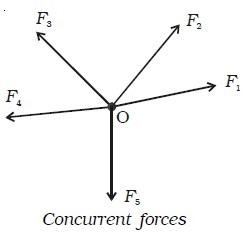
\includegraphics[scale=0.5]{concurrent coplanar force system.jpg}
	\label{fig:CCFS}
\end{figure}

\subsection{Parallelogram Law of Vector Addition}

The Parallelogram Law of Vector Addition is law that helps us to resolve a given vector into its respective components, or find the resultant of 2 vectors inclined to each other at an angle. 

It States that: 

\textit{"If two vectors acting simultaneously at a point can be represented both in magnitude and direction by the adjacent sides of a parallelogram drawn from a point, then the resultant vector is represented both in magnitude and direction by the diagonal of the parallelogram passing through that point."}

\begin{figure}[H]
	\centering
	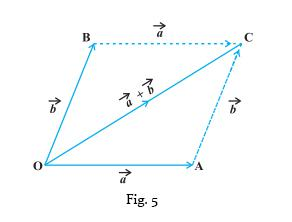
\includegraphics[scale=0.5]{Parallelogram law.jpg}
	\caption{Parallelogram Law of Vector Addition}
	\label{fig:Parallelogram law}
\end{figure}

\subsection{Polygon Law of Vector Addition}

Polygon law of vector addition states that: \\

\textit{If a number of vectors can be represented in magnitude and direction by the sides of a polygon taken in the same order, then their resultant is represented in magnitude and direction by the closing side of the polygon taken in the opposite order.}

\begin{figure}[H]
	\centering
	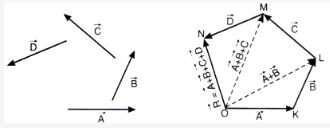
\includegraphics[scale=0.7]{polygon law.jpg}
	\caption{Polygon Law of Vector Addition}
	\label{fig: Polygon Law}
\end{figure}

\section{Procedure}
	\begin{enumerate}
		\item Find the Analytical Solution of the Given 3 Problems.
		\item Find the Graphical Solution of the Given 3 Problems by plotting to scale the figures and applying Polygon and Parallelogram Laws of Vector Addition. 
		\item Tabulate the Results
		\item Find the Error Percentage of the graphical Solution in comparison to the Analytical Solution using the formula:
		
		$$\mathrm{Percentage\ Error\ (\eta)} = \dfrac{|\mathrm{Graphical\ Value} - \mathrm{Analytical\ Value}|}{\mathrm{Analytical\ Value}} * 100$$
	\end{enumerate}
\pagebreak
\section{Analytical Method}


Q1. Find the Resultant of the Force system shown below. 
\begin{figure}[H]
	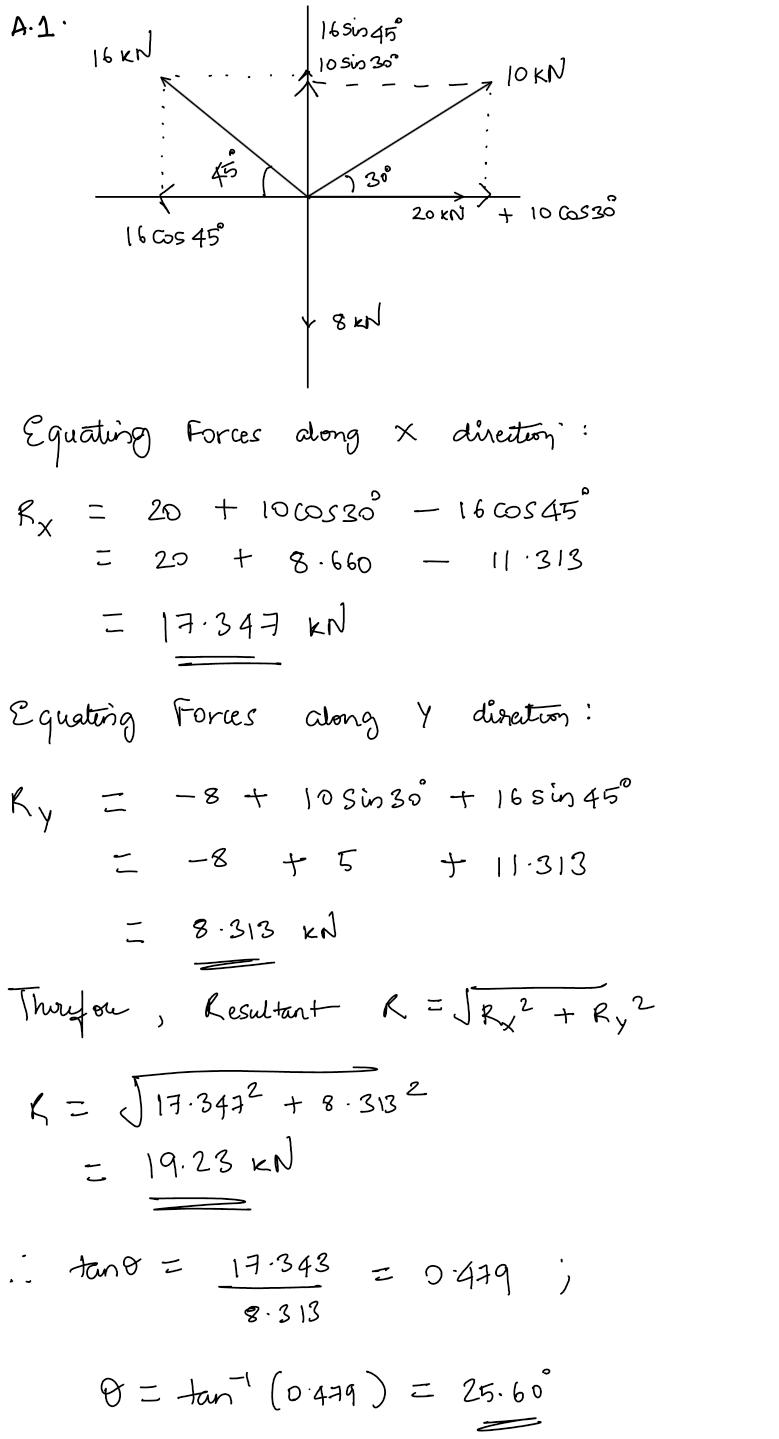
\includegraphics[scale=0.4]{a1.jpg}
	\label{fig: Polygon Law}
\end{figure}


\pagebreak
Q2. A 200 N force is to be resolved into components along lines a-a' and $ b-b' $ as shown in the figure. Determine the angle $\alpha$ knowing that the component along $ a-a' $ is to be 150N. What is the corresponding value of the component along $ b-b' $?
\begin{figure}[H]
	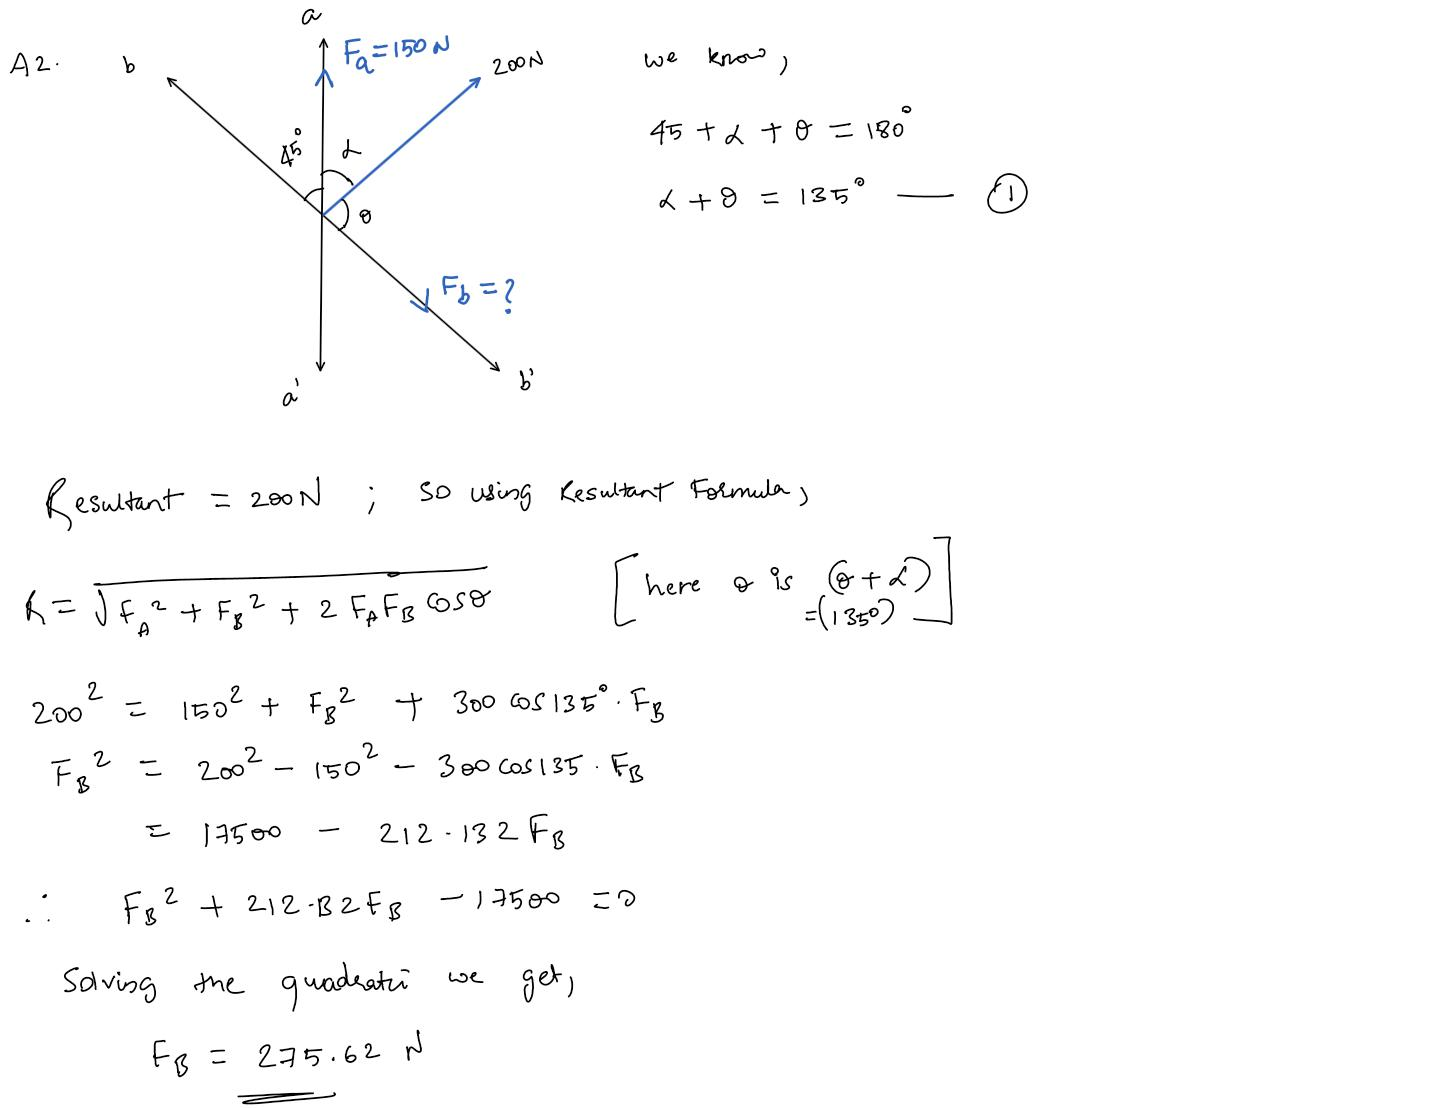
\includegraphics[scale=0.5]{a2.jpg}
	\label{fig: Polygon Law}
\end{figure}
\pagebreak
\begin{figure}[H]
	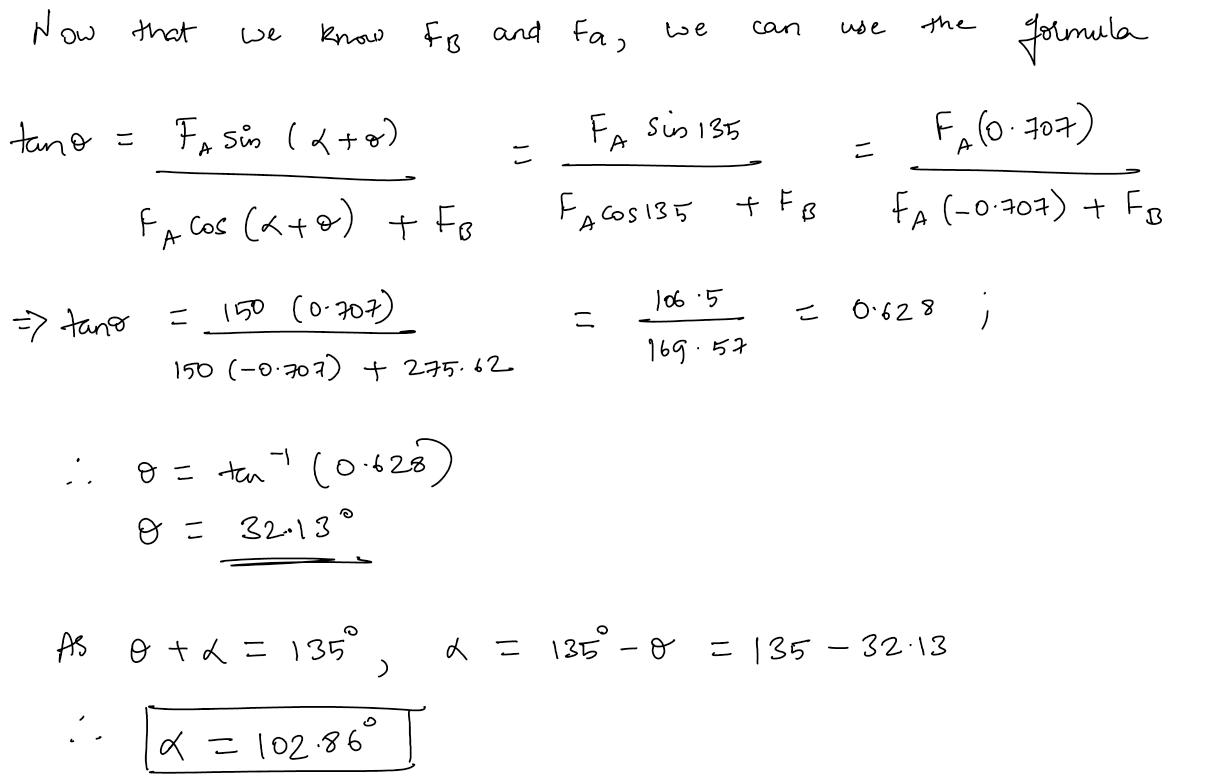
\includegraphics[scale=0.4]{a22.jpg}
	\label{fig: Polygon Law}
\end{figure}

\pagebreak

Q3. Under the action of five forces, the following system is in equilibrium. Determine the magnitude and direction of the fifth force. 

\begin{figure}[H]
	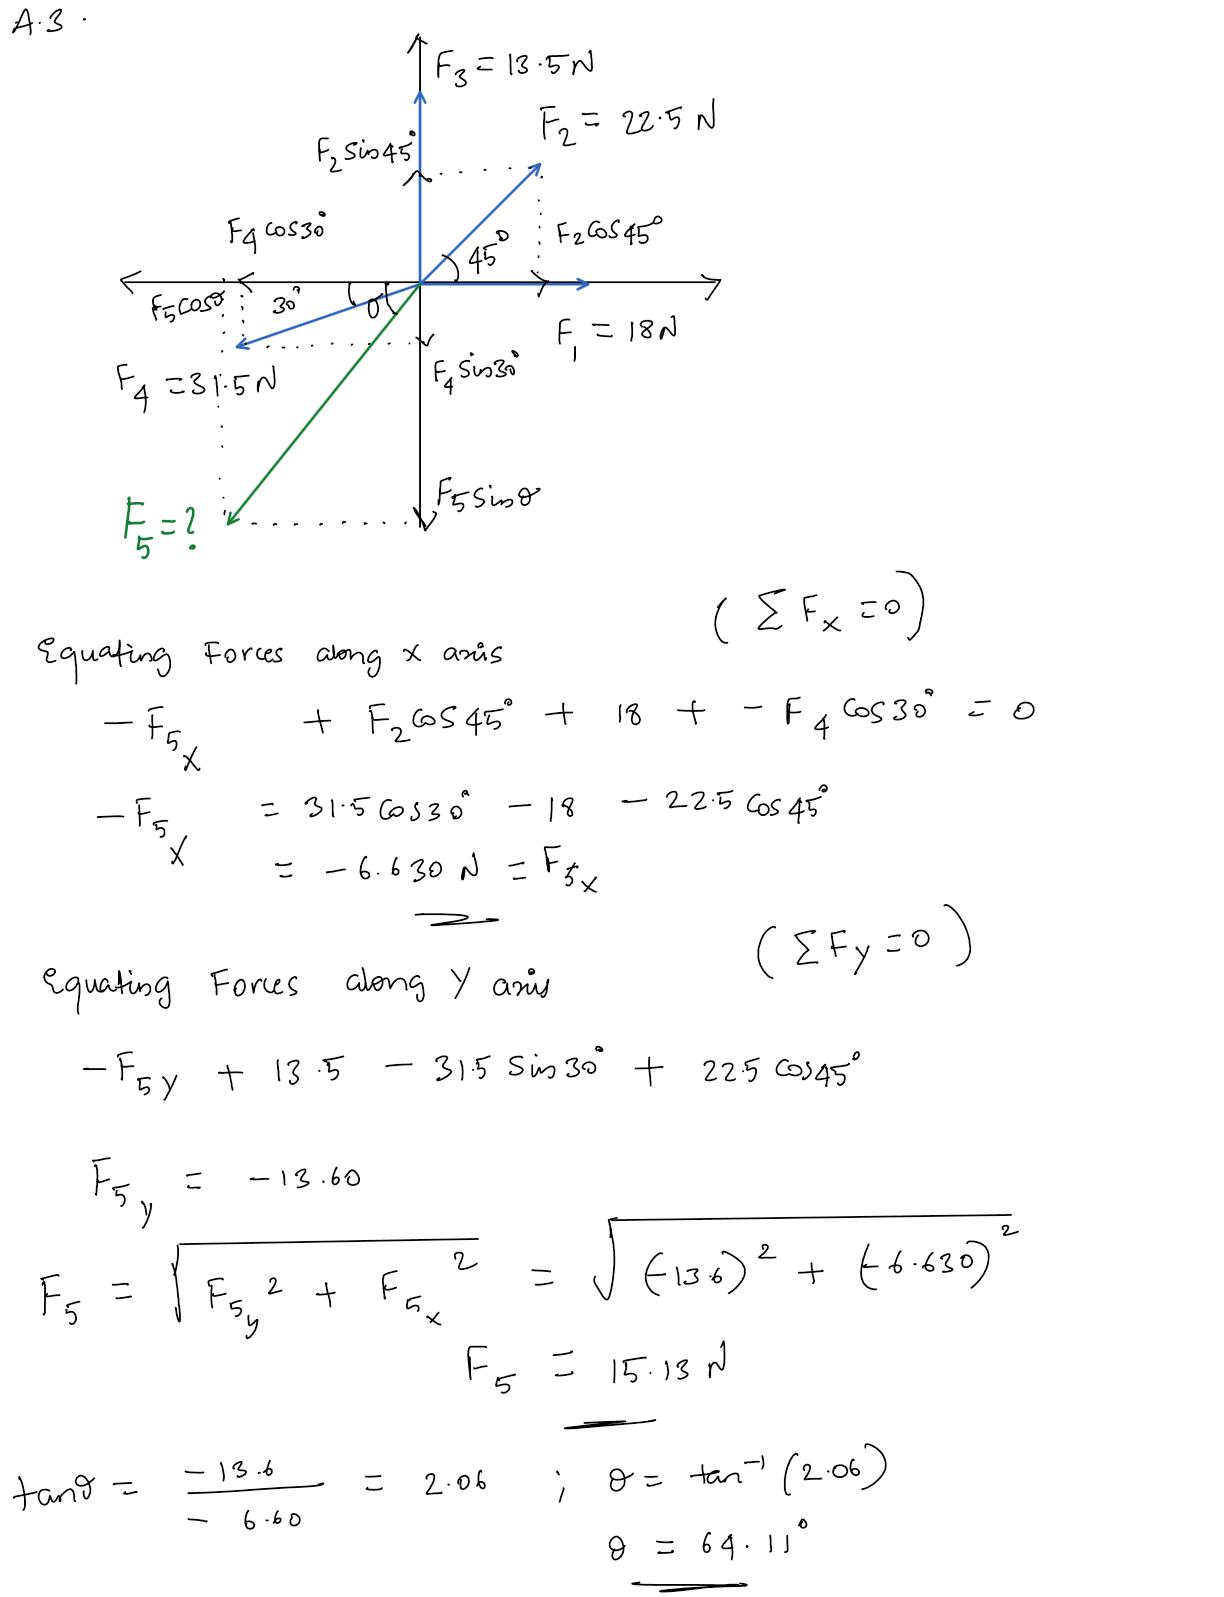
\includegraphics[scale=0.38]{a3.jpg}
	\label{fig: Polygon Law}
\end{figure}

\pagebreak

\section{Graphical Method}

Q1. Find the Resultant of the Force system shown below. 
\begin{figure}[H]
	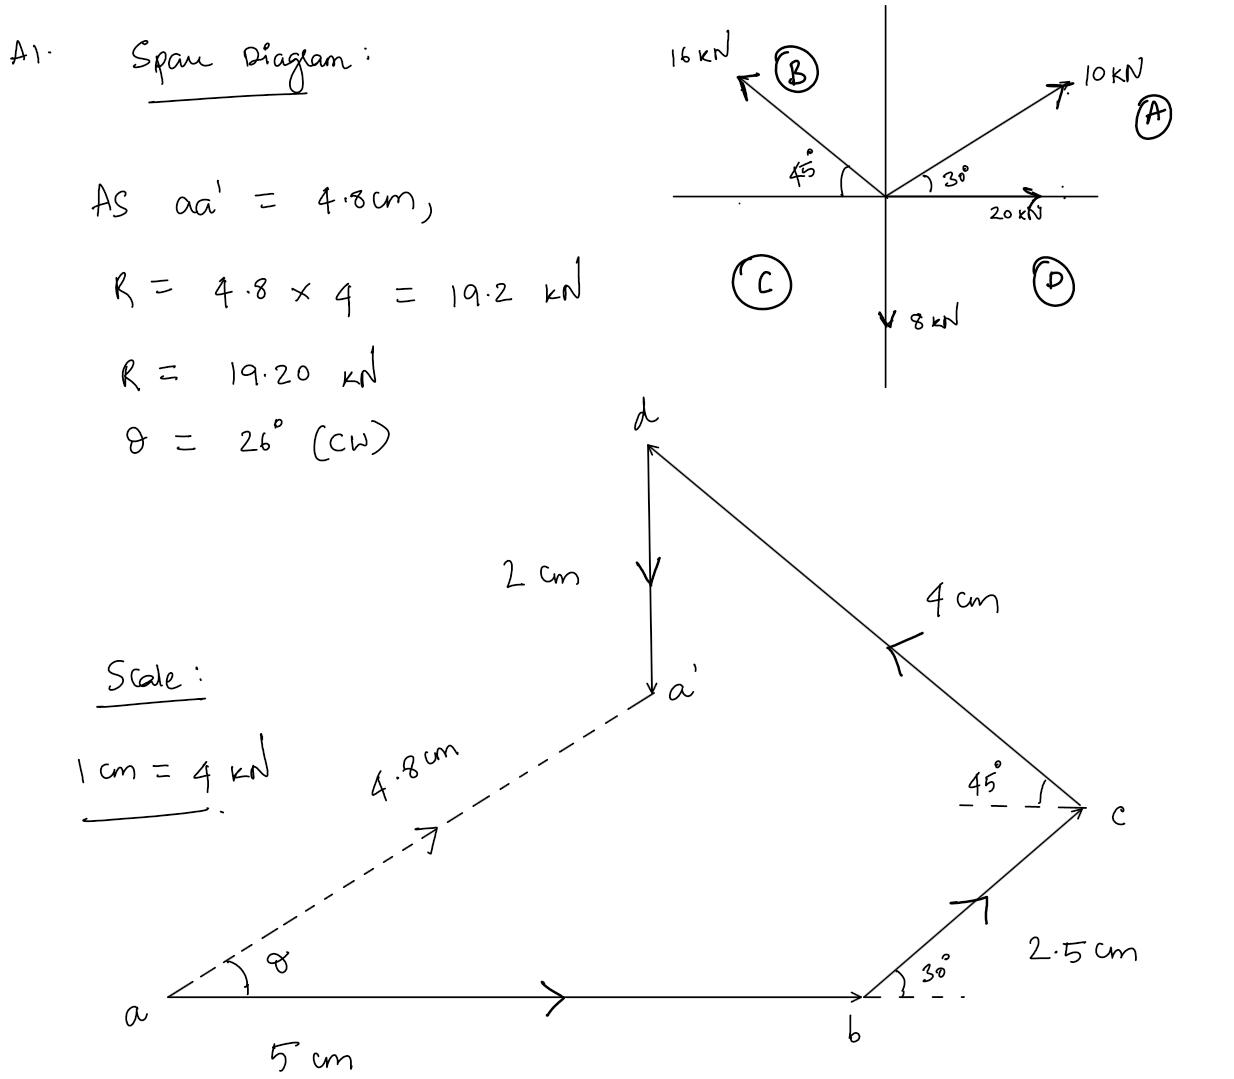
\includegraphics[scale=0.45]{g1.jpg}
	\label{fig: Polygon Law}
\end{figure}


\pagebreak
Q2. A 200 N force is to be resolved into components along lines a-a' and $ b-b' $ as shown in the figure. Determine the angle $\alpha$ knowing that the component along $ a-a' $ is to be 150N. What is the corresponding value of the component along $ b-b' $?
\begin{figure}[H]
	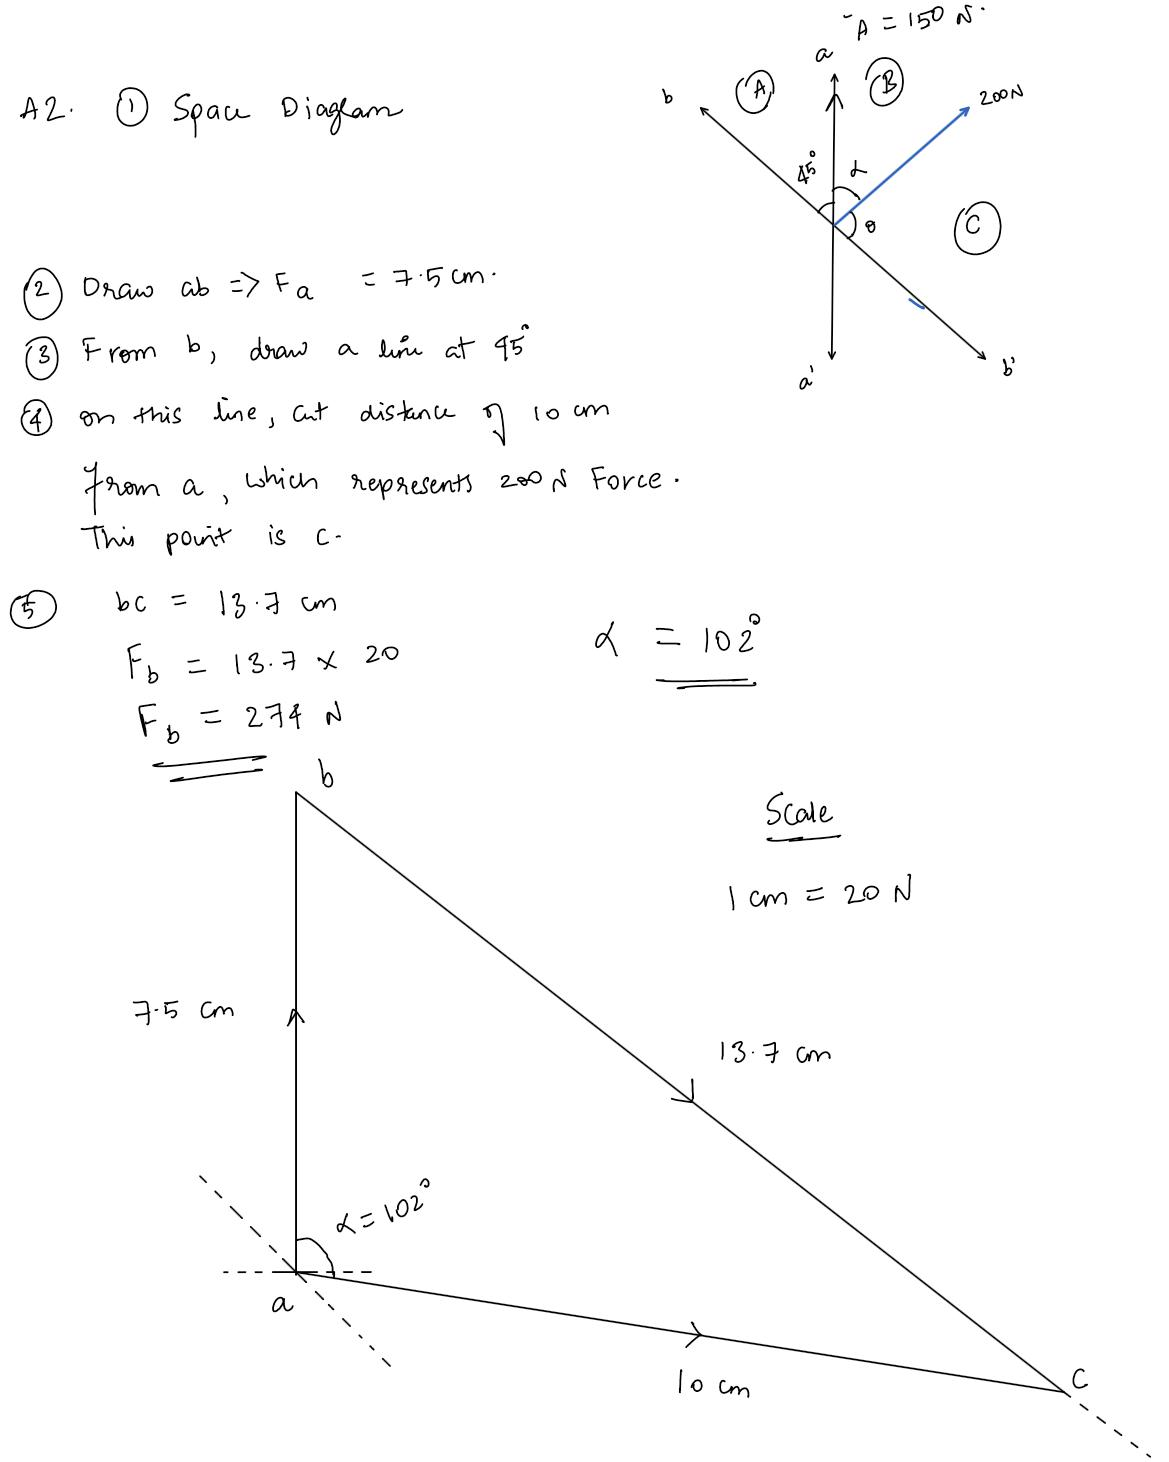
\includegraphics[scale=0.39]{g2.jpg}
	\label{fig: Polygon Law}
\end{figure}

\pagebreak

Q3. Under the action of five forces, the following system is in equilibrium. Determine the magnitude and direction of the fifth force. 

\begin{figure}[H]
	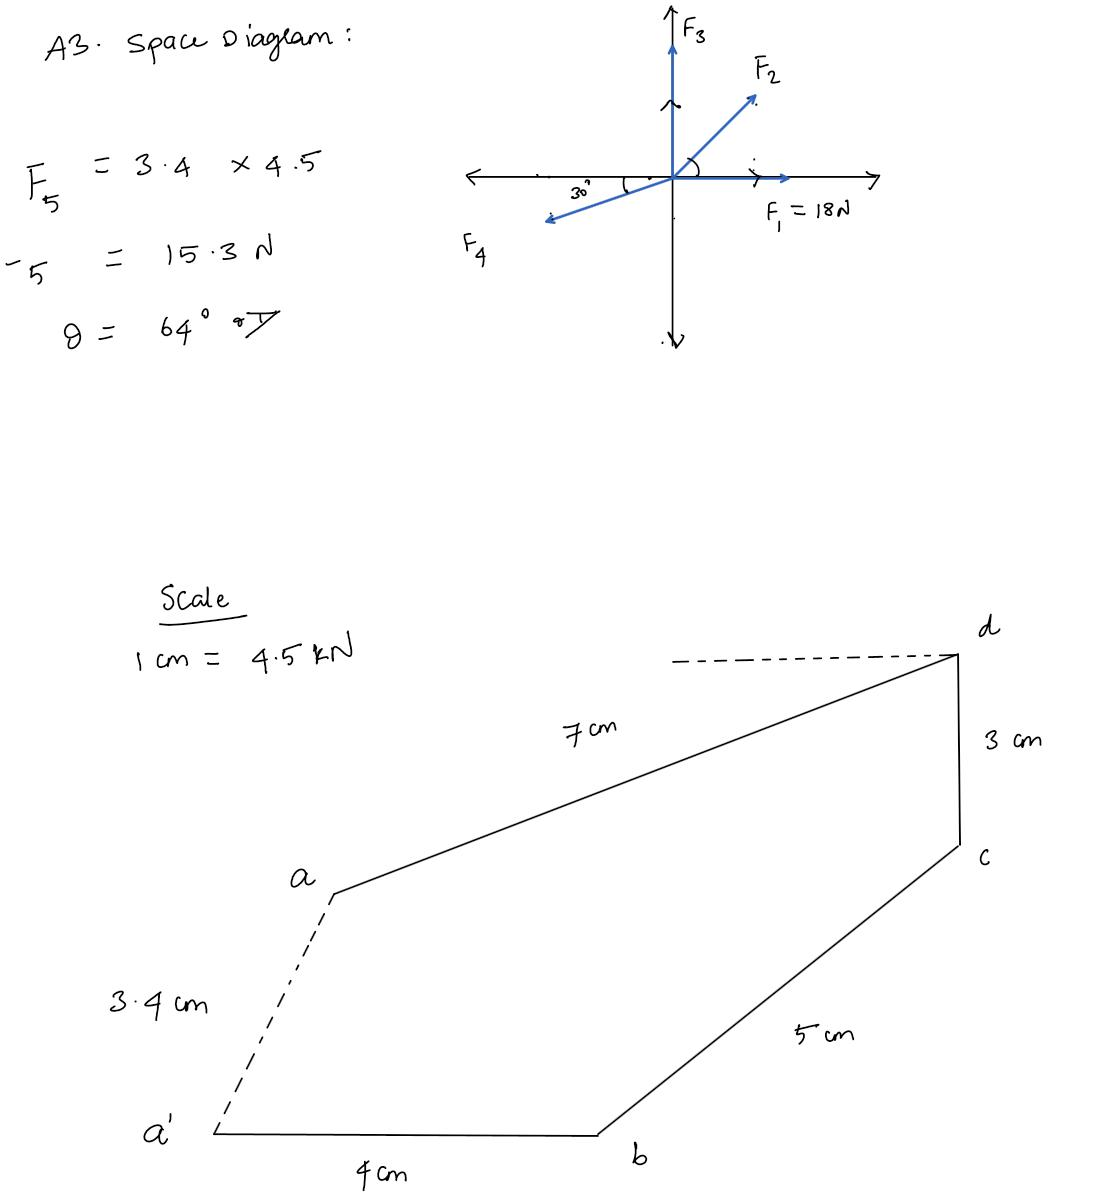
\includegraphics[scale=0.45]{g3.jpg}
	\label{fig: Polygon Law}
\end{figure}

\pagebreak

\section{Results}

\begin{tabular}{|c|c|c|c|}
	\hline
	Question Number & Analytical Solution & Graphical Solution & Percent Error \\
	\hline
	1 	& R = 19.23 kN  & R = 19.20 kN & $\eta_R = 0.31\%$\\
		& $\theta$ = 25.60$\degree$ & $\theta$ = 26.00 $\degree$ & $\eta_\theta = 1.56 \%$\\
	\hline
	2	& $ F_B = 275.62 N $ & $ F_B = 274.00 N $ & $\eta_{F_B} = 0.58\%$ \\
		& $ \alpha = 102.86\degree $ & $ \alpha = 102.00\degree $ & $\eta_\alpha = 0.83\%$ \\
	\hline
	3	& $ F_5 = 15.13 N $ & $ F_5 = 15.3 N $ & $\eta_{F_5} = 0.85\%$ \\
		& $ \theta = 64.11\degree $ & $ \theta = 64.00\degree $ & $\eta_\theta = 0.11\%$ \\
	\hline
\end{tabular}


\section{Conclusion}
A set of problems involving concurrent Co-planar Force system were solved using graphical as well as analytical methods. The Percentage error between the 2 answers was found.
\end{document}